%% Timing profile comparison summary
\section*{Timing Profile Comparison}
Exponential model: $t = a \cdot e^{b n}$, where $t$ is time (s) and $n$ is atom count.
\begin{table}[ht]
\centering
\begin{tabular}{lrrrrr}
\toprule
Profile & $a$ (s) & $b$ (atoms$^{-1}$) & $R^2$ & Mean (ms) & Median (ms) \
\midrule
All metrics & 8.40e-02 & 0.0057 & 0.9049 & 266.4 & 26.5 \
No resistance & 8.06e-02 & 0.0056 & 0.9094 & 249.4 & 25.8 \
No metrics & 5.54e-02 & 0.0058 & 0.9010 & 179.8 & 24.9 \
\bottomrule
\end{tabular}
\end{table}
\begin{figure}[ht]
\centering

\includegraphics[width=0.95\linewidth]{reports/timing_profiles_comparison.png}
\caption{Timing comparison across profiles with exponential fits.}
\end{figure}
\begin{figure}[ht]
\centering
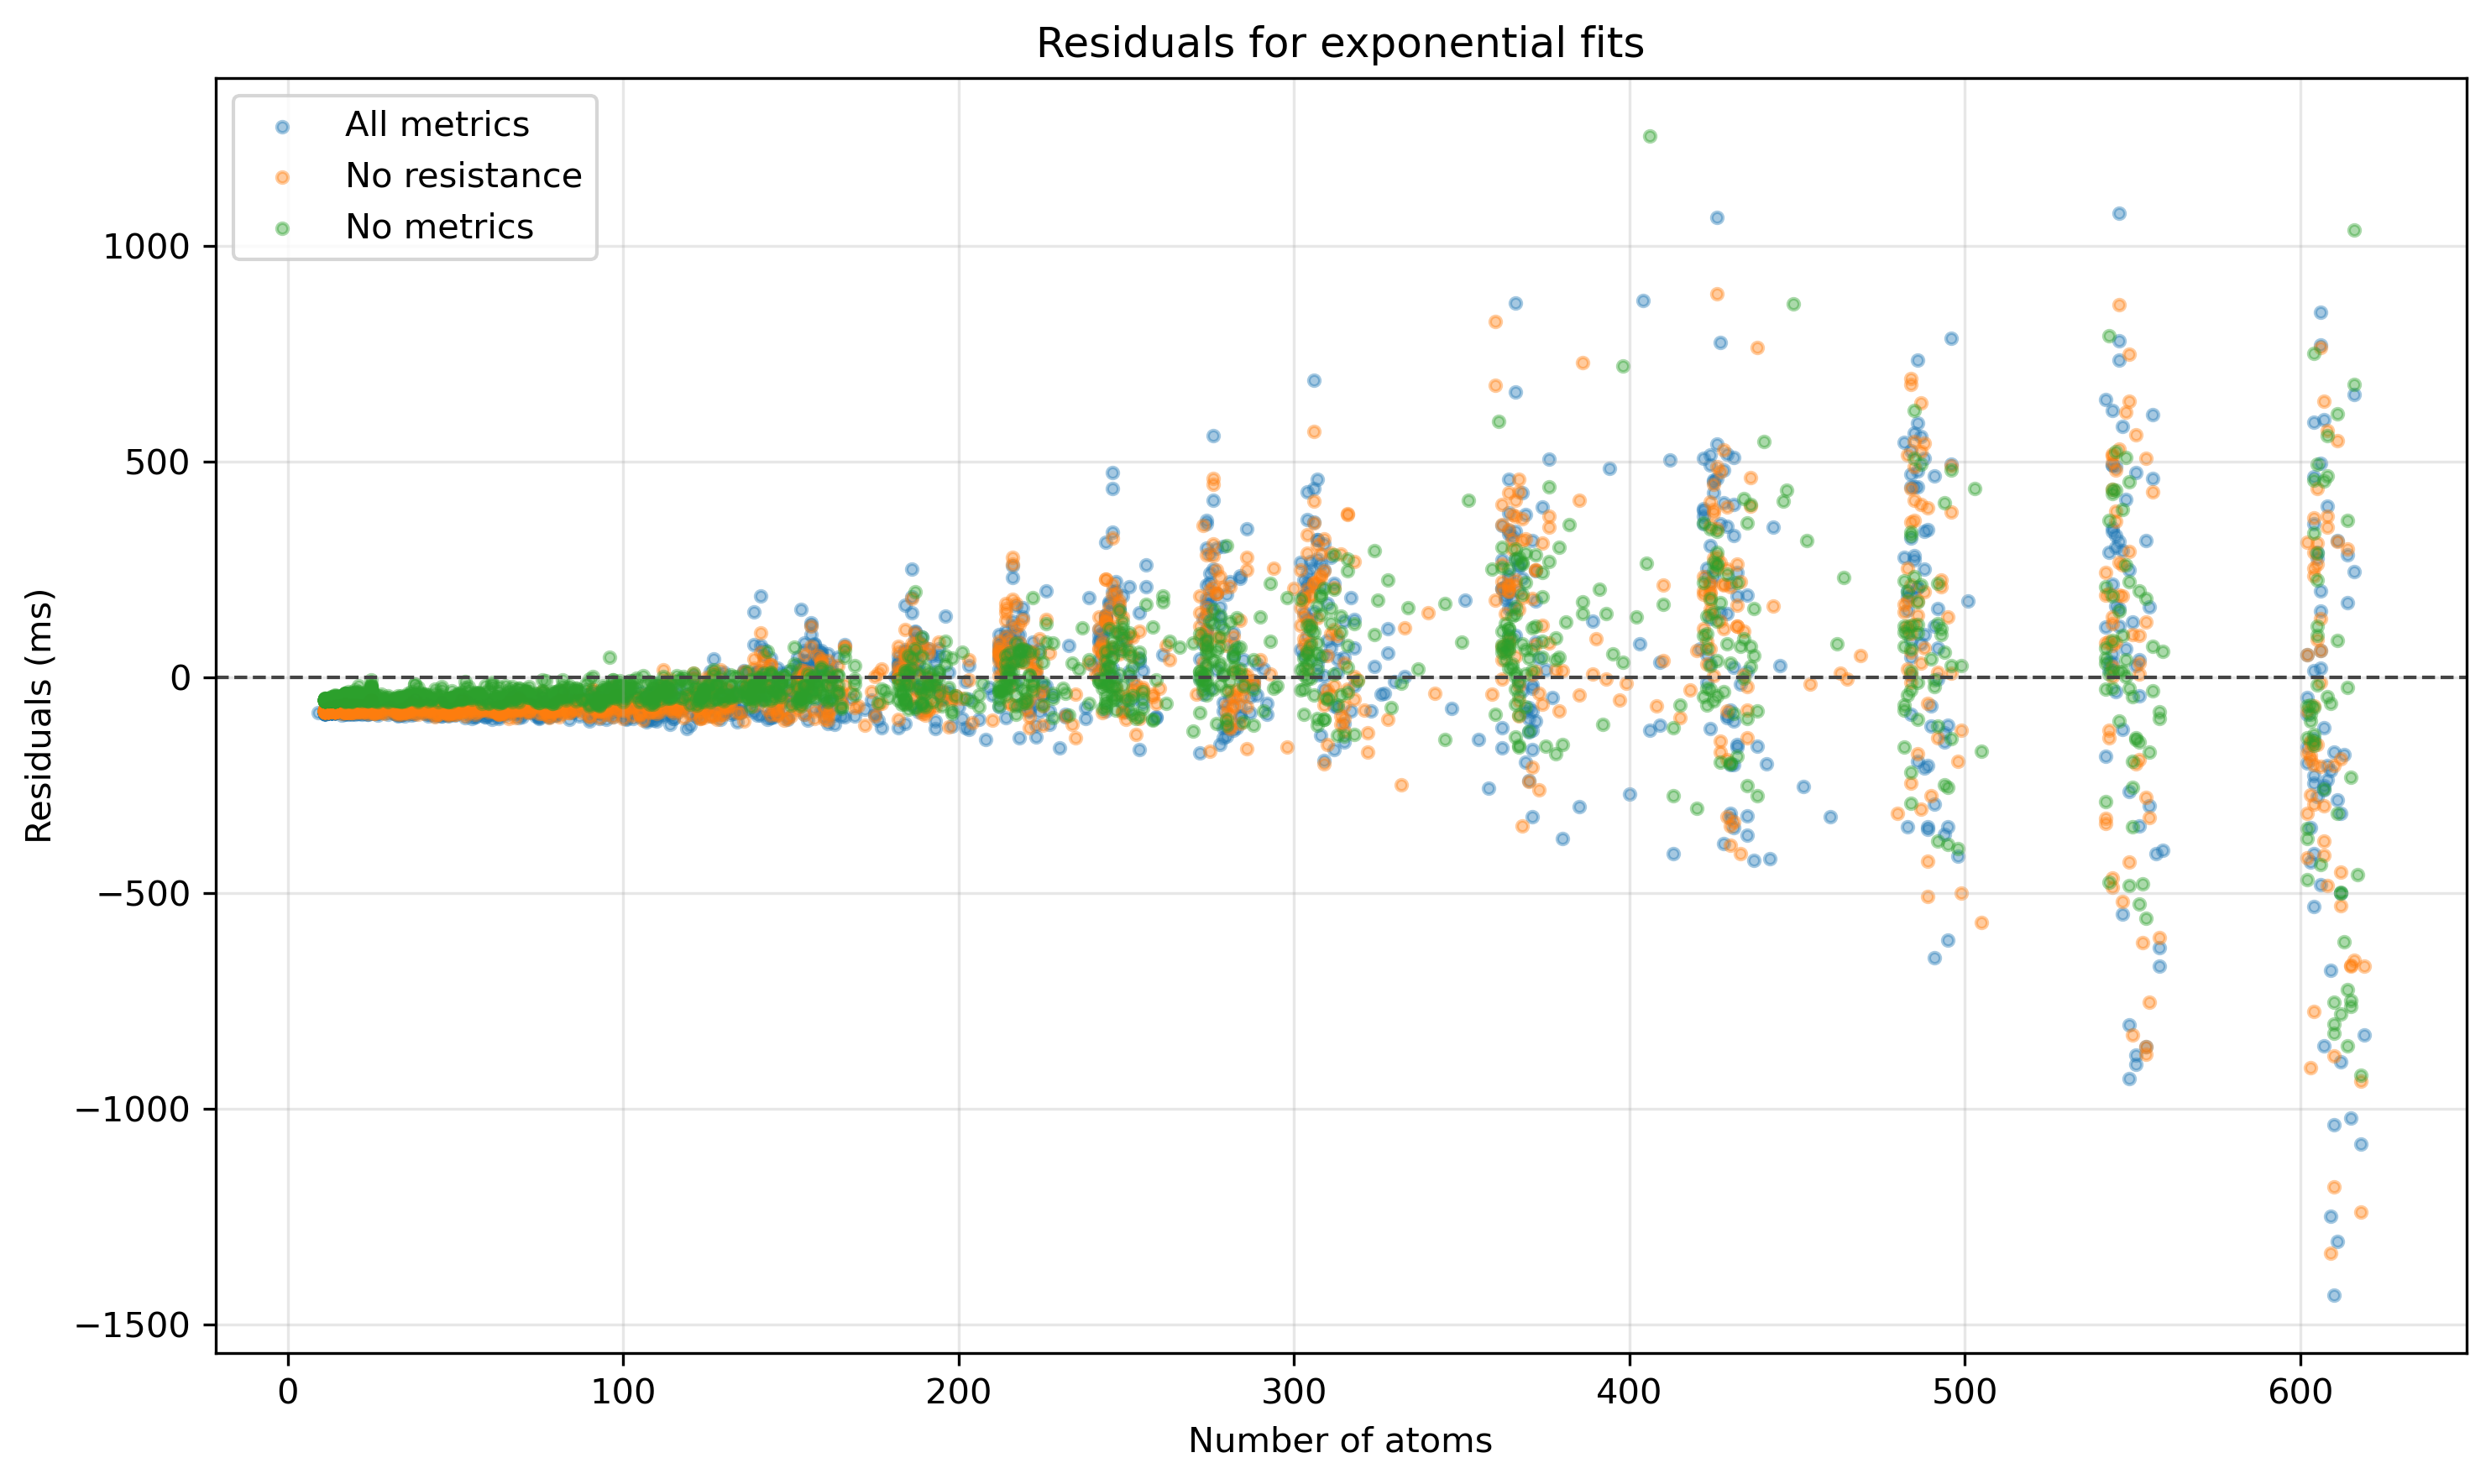
\includegraphics[width=0.95\linewidth]{reports/timing_profiles_residuals.png}
\caption{Residuals for exponential fits across profiles.}
\end{figure}